\section{Fundamentos de Comunicação de Dados em Rede}
Segundo \nocite{gallo2003comunicaccao}GALLO (2003), uma rede é um conjunto de sistemas que possuem uma forma de comunicação entre si com o objetivo de compartilhar informações.

Como exemplo, podemos citar a rede de telefonia. Cada telefone desta rede possui ligação com qualquer outro telefone - desde que você saiba o seu número. Basta você discar o telefone de uma pessoa e com isso você estabelecerá uma conexão entre o seu telefone e o telefone dela. Os dois aparelhos irão mandar dados uns para os outros - no caso, a conversa entre você e a pessoa do outro lado da linha.

Outro exemplo é a televisão. Os programas de televisão também chegam à você por meio de uma rede. Mas esta possui características bem diferentes das redes de telefonia. Nela não se pode enviar informações para as emissoras de televisão. Somente elas transmitem informações, para você e para milhares de outras pessoas.

	\subsection{História das Tecnologias de Rede}
	Uma rede de computadores envolve a interconexão entre dois ou mais micros, o que permite a troca de dados entre essas unidades e otimiza os recursos de hardware e software. Deve ter regras básicas que garantam o envio seguro de informações. Para ser eficiente, ela precisa que os dados transitem de um computador para outro sem que sofram danos. Também é necessário que a rede seja capaz de determinar corretamente para onde as informações estão indo. Além disso, os computadores interligados tem que poder se identificar uns aos outros e deve existir um modo padronizado de nomear e identificar as partes que a compõem. Atualmente, existem milhões de máquina conectadas à Internet e ela tornou-se tão poderosa que é capaz de transmitir entre computadores todo o tipo de dados como imagens, sons, vídeos, textos escritos e até mesmo programas de computador. \cite{forouzan2009comunicaccao}.
	
	\subsection{Conceitos Sobre Redes}
	Redes de Computadores formam uma tecnologia de rede única. Nenhuma outra tecnologia de rede é tão versátil e poderosa como ela. \cite{morimoto2006}. Devido à isso, quando falamos sobre elas, podemos utilizar os seguintes termos:
	\begin{description}
		\item[Clientes] são computadores que se conectam à um computador central para requisitar que este realize alguma tarefa na qual é especializado.
		\item[Confiabilidade] Em todo o tipo de comunicação à distância, existe a possibilidade de ocorrer um erro na hora de se interpretar os dados. No caso das redes de computadores, isso é algo que pode ocorrer devido à vários motivos como interferência ou o enfraquecimento do sinal com a distância. Para se criar uma rede de computadores confiável, é preciso fazer com que os computadores sejam capazes de detectar erros na transmissão. Uma vez que isso ocorra, pode-se tentar corrigí-los ou então pedir para que os dados sejam retransmitidos.
		\item[Endereço] para que possamos nos comunicar com outro elemento de uma rede, precisamos identificá-lo de alguma forma. Na rede telefônica, por exemplo, para falarmos com outra pessoa, precisamos discar o seu número de telefone - que é único para cada elemento da rede. O mesmo ocorre com a rede de computadores. Cada elemento possui um número único que é reconhecido como seu "Endereço". Quase todos os elementos de uma rede de computadores possuem um endereço. Chamamos o ato de distribuir Endereços para os elementos da rede de Endereçamento.
		\item[Meio] É o ambiente físico usado para conectar membros de uma rede. Por exemplo, no caso dos telefones, o meio é o fio que forma toda a rede telefônica. Computadores podem usar os mais diversos meios, como cabos e ondas de rádio.
		\item[Nó] Não são apenas computadores que podem ser ligados à uma rede de computadores. de fato, as primeiras redes de computadores foram criadas para controlar o caminho percorrido por ligações telefônicas. Existe uma gama muito grande de dispositivos que podem fazer parte deste tipo de rede como terminais, impressoras, repetidoras, pontes, chaves e roteadores. Por causa disso, costumamos chamar cada elemento conectado à uma Rede de Computadores de "Nó".
		\item[Protocolo] Computadores só podem lidar com números binários. Eles só entende 0s e 1s. Por conta disso, é preciso criar algum tipo de alfabeto ou padrão para que possamos nos comunicar com apenas dois tipos de sinais. O nome das regras que os computadores seguem para se comunicar entre si chama-se "Protocolo".
		\item[Roteamento] Rotear significa traçar uma rota. O roteamento é justamente a tarefa de traçar rotas entre os vários elementos de uma rede. Afinal, em uma rede com várias máquinas, é preciso estabelecer qual caminho os dados precisam seguir para que eles não terminem indo parar na máquina errada.
		\item[Segurança] É comum que informações sigilosas sejam trocadas em uma rede. Por causa disso, existem muitas pessoas que podem tentar interceptar os dados. Para isso, pode-se utilizar várias estratégias para aumentar a segurança de uma rede como criptografar os dados, por exemplo.
		\item[Servidor] Um Servidor é uma máquina que costuma ser freqüentemente acessada por outras para que ela realize algum tipo de tarefa.
	\end{description}

	\subsection{Classificação de Redes}
	Quanto ao Tamanho das redes, \cite{ross2009redes} diz que podemos classificá-las como:
	\begin{description}
		\item[PAN] O alcance destas redes normalmente é o de alguns poucos metros.
		\item[LAN] Qualquer rede cujo raio de alcance seja menor do que 10 Km se encaixa nesta categoria.
		\item[MAN] Este nome é usado para redes maiores do que LANs e que normalmente ocupam a área de uma cidade inteira. Embora existam MANs que pertencem à uma única organização, o mais normal é que elas sejam formadas por redes interconectadas de vários indivíduos e organizações diferentes. Elas também podem ser usadas pela administração do município como serviços de utilidade pública.
		\item[WAN] Qualquer rede cuja área é maior do que uma cidade se encaixa nesta categoria. Existem WANs que possuem uma área de alcance que cruzam até mesmo diferentes estados e países. Atualmente, a maior WAN existente é a Internet.
	\end{description}

	\subsection{Espaço de Redes}
	Segundo \cite{farias2006essncial}, o espaço de uma rede mostra como as máquinas estão ligadas entre si. Dessa forma as redes podem ser classificadas em:
	\begin{description}
		\item[Redes Ponto-a-Ponto] Em redes deste tipo, cada nó só pode se comunicar com nós adjacentes. É como em uma brincadeira de telefone sem fio no qual para que uma mensagem chegue até alguém, ela precisa passar por vários intermediários, já que só é possível falar com as pessoas que estejam ao seu lado.
			\begin{description}
				\item[Estrela] Neste tipo de rede, existe um nó central (normalmente um hub ou switch) à partir do qual todas as máquinas estão conectadas. Para enviar uma mensagem à alguém, é preciso primeiro enviar para o nó central e só então o nó central passa a mensagem para o destinatário.
					\begin{figure}[!htb]
						\centering
						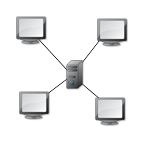
\includegraphics{img/estrela.jpg}
						\caption{Rede Ponto-a-Ponto Estrela}
						\label{Rede Estrela}
					\end{figure}
				\item[Laço] Neste tipo de rede, não existe um nó central. Ao invés disso, as máquinas então todas conectadas entre si e existem nós que estão conectados a mais de um outro nodo. Por não possuírem um nó central, não existe um único ponto cujo funcionamento mantém a rede inteira. Por isso, eles tendem a ser mais seguros. Entretanto, o roteamento neste tipo de rede tende a ser mais complexo. Existem também redes em laço que são totalmente conectadas. Nelas, cada nó está conectado à todos os demais. Por causa de sua complexidade e custo proibitivo, este tipo de laço só é usado em redes pequenas com poucos nós.
					\begin{figure}[!htb]
						\centering
						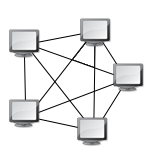
\includegraphics{img/laco.jpg}
						\caption{Rede Ponto-a-Ponto Laço}
						\label{Rede Laço}
					\end{figure}
				\item[Árvore] Neste tipo de topologia, existe um nó que é considerado a raiz. Ela possui ligada à ela outros nós que são considerados seus filhos e ele é o pai destes nós. Cada nó que é filho da raiz pode ter outros filhos e estes também podem ter seus filhos. Entretanto, cada nó, com exceção da raiz, deve possuir um único pai. Normalmente, estas redes possuem como nós diversos Hubs ou Switchs. Nelas, os nós que não possuem filhos normalmente são os computadores e terminais de trabalho.
					\begin{figure}[!htb]
						\centering
						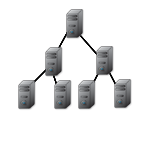
\includegraphics{img/arvore.jpg}
						\caption{Rede Ponto-a-Ponto Árvore}
						\label{Rede Árvore}
					\end{figure}
			\end{description}
		\item[Redes de Difusão] Neste tipo de rede, os nós compartilham um canal único de comunicação. Nele, os dados enviados por uma máquina são recebidos por todos os nós que compartilham um mesmo canal. É como em uma conversa normal. Quando você fala, várias pessoas ao redor ouvem o que você disse, mas somente a pessoa com quem você está falando responde.
			\begin{description}
				\item[Barramento] Neste tipo de rede, todos os nós compartilham um mesmo canal. Se algum dos nós enviar uma mensagem pela rede, todos os demais irão ouvir. Deve-se tomar cuidado para que mais de um nó não tente falar ao mesmo tempo, pois se isso ocorrer, ninguém conseguirá entender a mensagem transmitida.
				\begin{figure}[!htb]
					\centering
					
\includegraphics{img/barramento.jpg}
					\caption{Rede de Difusão Barramento}
					\label{Rede Barramento}
				\end{figure}
				\item[Satélite] Segundo \cite{torres2015redes}, neste tipo de rede, existe um satélite capaz de transmitir dados para todos os nós em Terra que estejam na área de alcance e estejam equipados com antenas para captar o seu sinal. Se o satélite envia um sinal, todos os outros nós ouvem. Mas se um nó mandar uma mensagem para o satélite, somente o satélite será capaz de ouvir a mensagem.
			\end{description}
	\end{description}

	\subsection{Método de transmissão de dados}
	\begin{description}
		\item[Comunicações Paralelas e em Série:] \cite{castells2002sociedade} diz que a comunicação serial é o método de transmissão de dados no quail cada símbolo que compõe a mensagem é mandado um de cada vez. Por contraste, comunicação paralela é toda aquela na qual um grupo de símbolos é enviado simultaneamente.
		
		A comunicação paralela é muito mais rápida, mas ela possui um problema grave. É preciso garantir que cada bit enviado chegue sempre de forma simultânea aos demais. Se ocorrer atrasos em somente um dos bits, ocorre erro de transmissão e a mensagem precisa ser corrigida ou enviada novamente. Isso acaba diminuindo a velocidade de transmissão. Quanto maior a distância percorrida pelos bits, mais difícil é garantir a sincronia. Atualmente, a comunicação paralela é utilizada principalmente em circuitos internos do computador e em HDs convencionais embora ela já tenha sido usada em impressoras e periféricos antigos.
		
		A comunicação serial é muito mais confiável e seus problemas com velocidade vem sendo superados com novas tecnologias. Atualmente ele é usado em HDs SATA, redes, fibras óticas, mouses e teclados USB e USB 2.0.
		
		\item[Comunicações Síncrona, Assíncrona e Isócrona] Quando enviamos um dado por meio de uma comunicação serial, é preciso haver uma forma de identificarmos onde começa e onde termina cada trecho da mensagem. Por exemplo, se eu enviar a mensagem o caractere H, seguido de um caractere A para um outro computador na rede, como aquela outra máquina saberá onde começa o "H" e onde começa e termina o "A" se tudo o que ele recebeu foi uma quantidade enorme de 1s e 0s?
		
		Uma das formas é enviar os dados de forma síncrona. Com isso, eu só posso enviar dados em períodos de tempo pré-determinados. Desta forma, eu envio um "H", aguardo um período de tempo pré-determinado e só então envio o "A". Caso eu não queira enviar nada, de tempos em tempos eu devo enviar uma seqüência de bits que representa que eu não estou falando nada. É assim que funcionam as mensagens enviadas por celulares, por exemplo.Nós só não percebemos isso quando falamos por meio deles porque o intervalo de envio de dados de um celular é muito curto.
		
		Outra solução para o problema seria antes de enviar qualquer coisa, enviar uma seqüência de bits que marcasse o início de uma transmissão e, após terminar, enviar bits que representem o fim da transmissão. O nome que damos à isso é "encapsulamento de dados". A vantagem é que assim eu posso enviar dados à qualquer momento. Além disso, a comunicação assíncrona é mais barata, por não exigir que hajam relógios no hardware monitorando a chegada de dados. Mouses, teclados, HDs e praticamente 99% dos dispositivos existentes hoje em dia utilizam este método de transmissão.
		
		Outro método de transmissão é a isócrona. Nela, envia-se mensagens ininterruptamente e o intervalo entre uma mensagem e outra já é conhecido e não muda nunca. Isso é normalmente usado para transmitir sinais de televisão digitais e também para aparelhos projetados para mostrar vídeos. Ela ainda é pouco usada, mas seu uso tende a ser maior à medida que surgem mais tecnologias que convergem vídeo, voz e dados em um mesmo meio de comunicação.
		
		\item[Comunicação Analógica e Digital] A comunicação analógica ocorre quando usamos para nos comunicar algum tipo de sinal físico que pode variar de forma contínua em quantidade ou força. A voltagem de uma corrente elétrica - por exemplo. Normalmente dispositivos analógicos fazem com que a intensidade ou voltagem de uma corrente elétrica oscile. Com isso, podemos usar a amplitude, frequência ou a fase da variação para transmitirmos dados. Também podemos usar todas estas coisas juntas. A comunicação analógica é utilizada em telefones fixos, celulares, modems, aparelhos de fax, TVs à cabo, rádio e outros.
	\end{description}
	














